\chapter{Deployment and Maintainence}

\section{Installation requirments}

\begin{enumerate}
\item Fuse - Linux kernel version 2.6.14+
\item GCC - version 4.6+
\item Sqlite3 - version 3.6+
\end{enumerate}

\section{Quick Start Guide}
\begin{enumerate}
\item Get the latest copy of KWEST form the project hosting site.
\item Make sure you have the mininum version of dependencies installed.
\item Compile the source using a standard C compiler.
\item Run the KWEST program which will mount the file system.
\item When required to unmount, use the fusermount command.
\end{enumerate}

\section{Uninstallation and Removal of data}
\begin{enumerate}
\item KWEST ``installs'' files in the users local directory.
\item To clean all the installation data including the database and log files, the user should use the \emph{make clean} or \emph{make ob} commands.
\item These commands are present in the Makefile, which comes with the project source.
\item In case of manual installation, there is a \emph{kwest} folder in the \emph{.config} directory.
\item Incomplete removal of files may cause haphazard execution of the program or corruption of files.
\end{enumerate}

\setcounter{section}{0}
\chapter*{User Manual}

KWEST is a virtual filesystem. This means that the folders and files represented by it are a part of its virtual organisation. Each file in KWEST represents an actual file stored somewhere on the underlying file system. The main focus of using KWEST is organisation.

\section{Installing}
\begin{itemize}
\item Once can get the latest copy of KWEST by downloading from the project hosting site: \url{https://code.google.com/p/kwest/downloads}
\item After extracting the contents, open up a terminal and type in the following commands:
\begin{lstlisting}[language=bash,frame=single]
make kwest_libs
export LD_LIBRARY_PATH=../lib:D_LIBRARY_PATH
make
\end{lstlisting}
\end{itemize}

\section{Mounting and Unmounting}

\begin{itemize}
\item To mount a KWEST filesystem, the user needs to run the \textit{mount} script which will mount the file system in the specified folder. 
\begin{lstlisting}[language=bash,frame=single]
./kwest mountpoint
KWEST - A Semantically Tagged Virtual File System
Initiating logging file(s).........
SUCCESS!
plugin loaded
name: taglib_audio
type: Audio
plugin loaded
name: pdfinfo
type: PDF
plugin loaded
name: extractor
type: Multiple
Importing file from /home/harsh/Music
Import completed SUCCESSFULLY
\end{lstlisting}
\item To unmount a KWEST filesystem, the user needs to run the \textit{fusermount -u} command with the argument \textit{path of KWEST mount point}. A successful unmount operation does not return any message.
\begin{lstlisting}[language=bash,frame=single]
fusermount -u mountpoint
\end{lstlisting}
\end{itemize}

\section{Importing Files and Folders}

\begin{itemize}
\item By default KWEST imports from the users \textbf{HOME} folder. It recursively scans all the subfolders and imports the folder hierarchy into KWEST. Hidden files are ignored by KWEST.

\item The user can also explicitly use the \textbf{import} tool to import files and folders into KWEST. The import tool accepts the folder to import as argument and imports all files and folders within it. It can work regardless of whether the KWEST file system is mounted or not.

\item While importing, the metadata of the file is used to organise each file. For e.g.: A music file contains the song's artist, which is used to categorise that file.
\end{itemize}

\section{Folder Structure}

The first layout when viewing a KWEST file system is called the Base folder. This folder contains a proper organisational view of the imported data, categorised by their metadata types. It contains the following folders:

\begin{figure}[htb]
\centering
\setlength\fboxsep{0pt}
\setlength\fboxrule{0.5pt}
\fbox{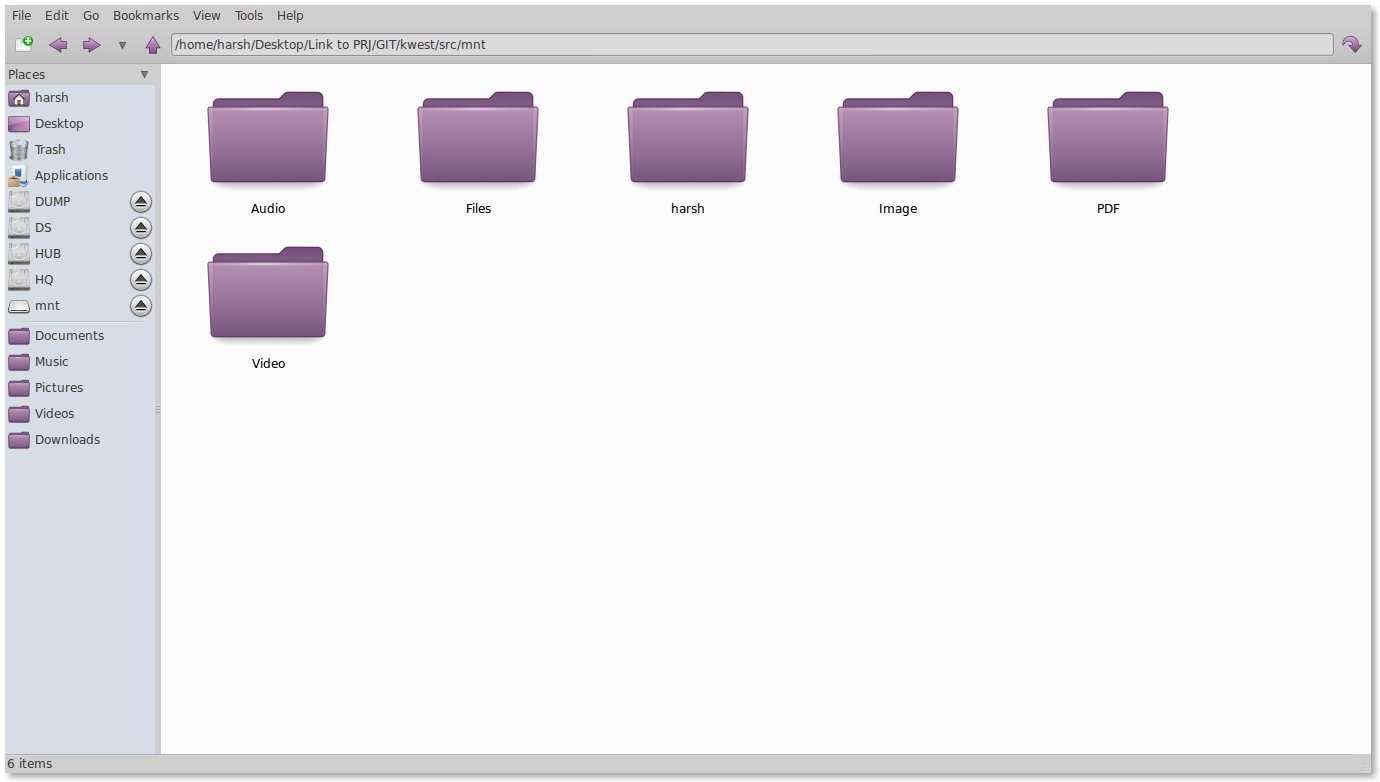
\includegraphics[width=0.8\linewidth]{./opimg/pcm_base.png}}
%\includegraphics[width=0.8\textwidth]{image.png}
\caption{KWEST file system view after mounting}
\label{fig:dfd0}
\end{figure}

\begin{enumerate}
\item \textbf{Files} \newline
This folder contains the user's folders as they  appear on their underlying file system. The folder is provided to give the user a quick access to their previous data organisation, as well as to demonstrate the superiority of a KWEST organisation.
\item \textbf{Audio} \newline
This folder contains all the files recognised by the system as being of type audio. Upon accessing the folder, each Audio file is further categorised by \textbf{Album}, \textbf{Artist}, \textbf{Genre}. If a particular metadata is absent for the audio file, KWEST categorises it in the Unkown folder. \newline
For e.g. If the audio file does not have any artist associated with it, it can be found in \textbf{UnknownArtist}.
\begin{figure}[htb]
\centering
\setlength\fboxsep{0pt}
\setlength\fboxrule{0.5pt}
\fbox{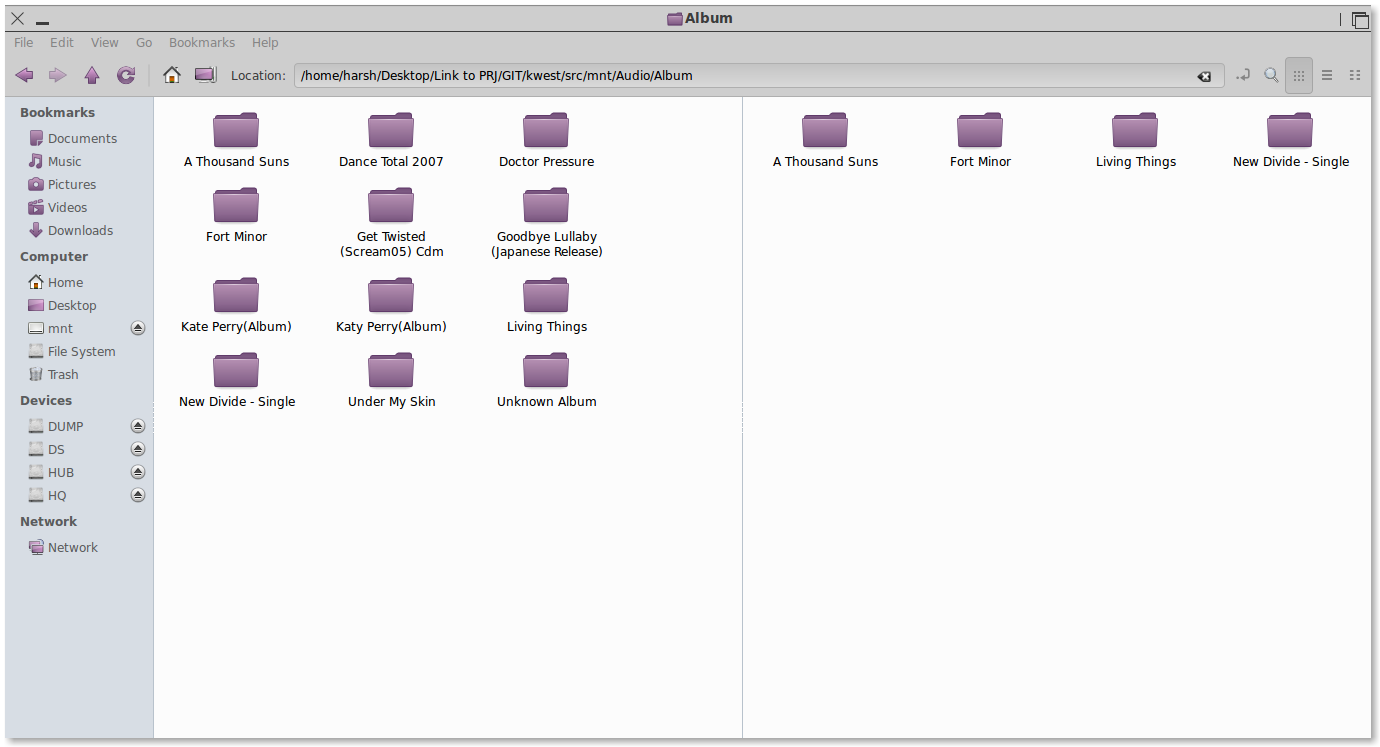
\includegraphics[width=0.8\linewidth]{./opimg/nemo_audiodual.png}}
%\includegraphics[width=0.8\textwidth]{image.png}
\caption{Audio files being categorised by /Album and /Artist/Album views}
\label{fig:dfd0}
\end{figure}

\item \textbf{Image} \newline
This folder contains all the image files recognised by the system. Inside, the images are organised by ImageCreator and ImageDate. 
The ImageCreator subfolder is based on \textit{Creators} like software - Adobe Photoshop, or hardware - Camera Models. Each ImageCreator tag is further organised by ImageDate. 
The ImageDate folder contains images sorted by \textit{Month-Year} of creation. Eg: A picture taken on ``\textit{2nd March 1992}'' will appear under ``\textit{1992Mar}''.
As with Audio, files with metadata missing will appear under appropriate \textit{Unkown} subfolders.
\begin{figure}[htb]
\centering
\setlength\fboxsep{0pt}
\setlength\fboxrule{0.5pt}
\fbox{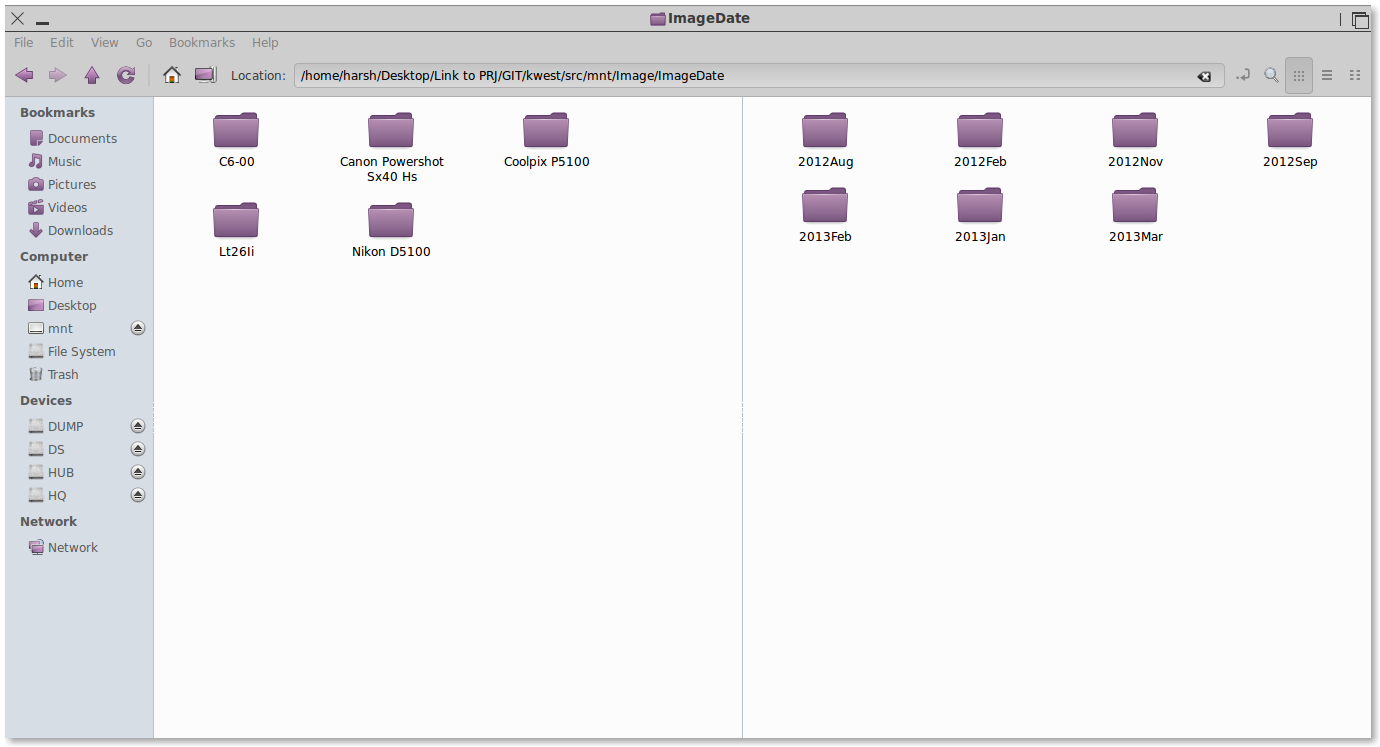
\includegraphics[width=0.8\linewidth]{./opimg/nemo_imagesort.png}}
%\includegraphics[width=0.8\textwidth]{image.png}
\caption{Images being categorised by Creator and CreationDate}
\label{fig:dfd0}
\end{figure}

\item \textbf{PDF} \newline
All PDF documents are tagged with the PDF tag. Each PDF document is organised by its \textit{Author,Publisher,Subject} and \textit{Title}. Files with metadata missing are appropriately tagged under \textit{Unknown} tags.
\begin{figure}[htb]
\centering
\setlength\fboxsep{0pt}
\setlength\fboxrule{0.5pt}
\fbox{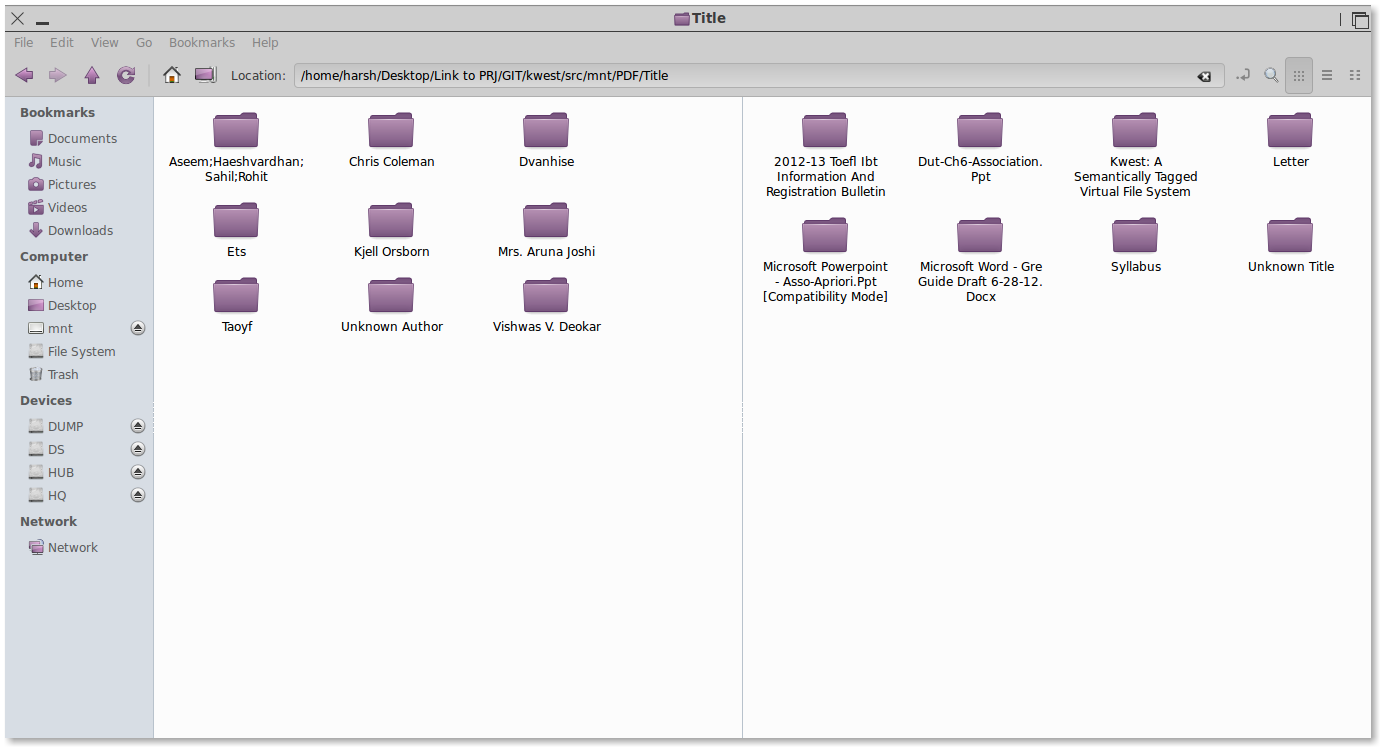
\includegraphics[width=0.8\linewidth]{./opimg/pdfsort.png}}
%\includegraphics[width=0.8\textwidth]{image.png}
\caption{PDF documents being seperated by Author and Title}
\label{fig:dfd0}
\end{figure}

\item \textbf{Video} \newline
Currently, the system organises video based only on Length, with the categories being \textit{Short, Medium and Long}. A short video is anything with less than 1800s of playtime. Videos with play time equal to or greater than 5400s are considered Long, and anything between them is considered Medium. The Video tag does not contain any categories as most of the videos stored by the user do not have any metadata present.
\begin{figure}[htb]
\centering
\setlength\fboxsep{0pt}
\setlength\fboxrule{0.5pt}
\fbox{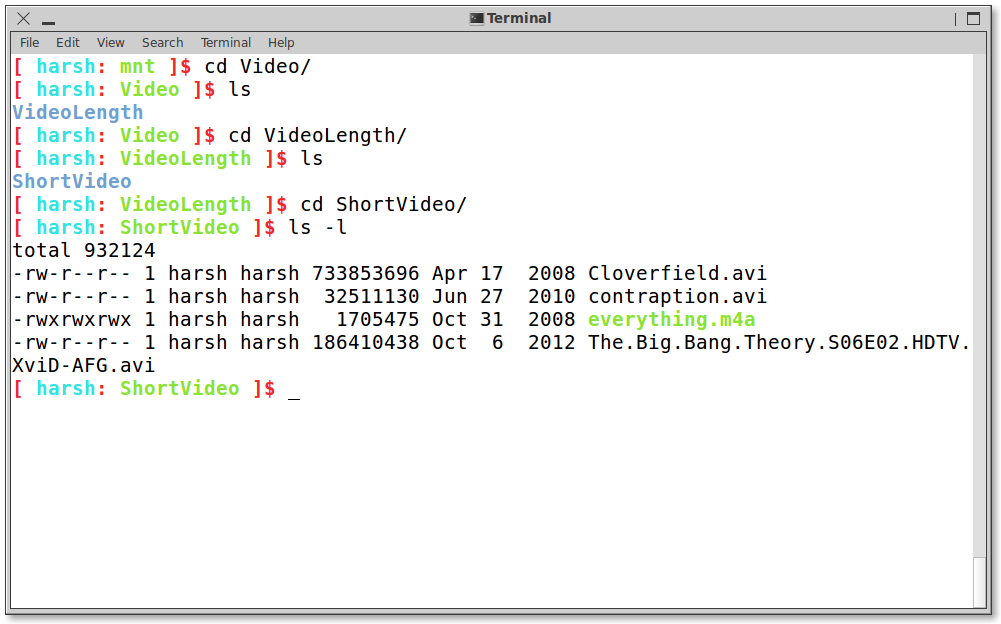
\includegraphics[width=0.8\linewidth]{./opimg/term_video.png}}
%\includegraphics[width=0.8\textwidth]{image.png}
\caption{Browsing the KWEST Video folder in a terminal}
\label{fig:dfd0}
\end{figure}

\item \textbf{`USER'} \newline
The tag \textbf{`USER'} refers to the \textit{username} of the current user. The user can create and manage his own personal tags in this folder.
\end{enumerate}
\begin{figure}[htb]
\centering
\setlength\fboxsep{0pt}
\setlength\fboxrule{0.5pt}
\fbox{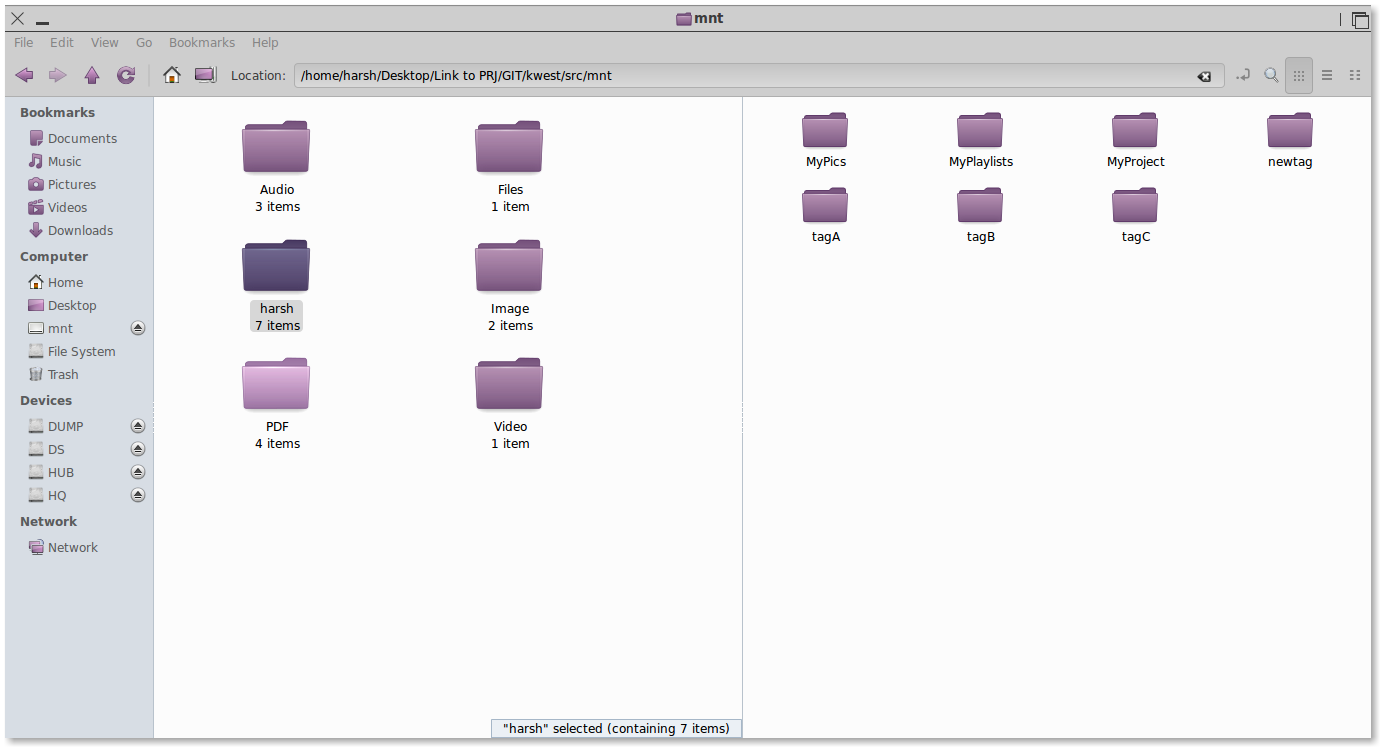
\includegraphics[width=0.8\linewidth]{./opimg/usertags.png}}
%\includegraphics[width=0.8\textwidth]{image.png}
\caption{User tags displayed in KWEST}
\label{fig:dfd0}
\end{figure}

\section{File System Operations}
The KWEST file system supports all common file system operations. One can read,write and execute files and programs as any traditional file system. Apart from these, KWEST features the following additional operations:

%Tag based operations
\subsection{Tags based:}
Tags are like keywords, or identifiers which help classify and identify date \textit{tagged} under them. 
In a KWEST file system, Tags are represented as virtual folders, which look, act and behave the same way as a normal folder.
\begin{itemize} 
%1. Tag a file
\item \textbf{Tag a file:} \newline
Tagging a file is an analogy for referencing the files by using tags. It is like accessing a piece of information using a keyword.
To tag a file, one simply ``\textit{copies}'' it under the appropriate tag. The normal copy operation is intepreted as \textit{tagging} operation in KWEST.
%2. Tag a tag
\item \textbf{Tag a tag:} \newline
Similar to tagging a file, a tag can also be tagged, creating multiple structures of organisation in the file system. To tag another tag, one simply creates a subfolder with the intended name, or copies the tagged folder to the location. \newline
e.g: to tag a folder called \textit{Pisces} under \textit{Zodiac}, one can create the folder /Zodiac/Pisces or copy Pisces into Zodiac.
%3. Rename a tag
\item \textbf{Rename a tag:} \newline
Renaming a tag will cause all instances of that tag  (which appear in other tags or views) to be renamed as well. So, for e.g. renaming the tag \textit{Zodiac} to \textit{SunSigns} will cause all instances of \textit{Zodiac} to now appear as \textit{SunSigns}.
%4. Delete a tag
\item \textbf{Delete a tag:} \newline
Deleting a tag will untag all files in it in the entire file system and will remove all instances of that tag from the database. 
\end{itemize}

%File based operations
\subsection{File based:}
\begin{itemize}
%1. Create a file
\item \textbf{Creating new files:}
As of now, KWEST is a tool for helping the users organize their files. Creating a new file is not yet a supported operations. However, users can create files on other file systems and import them into KWEST. Import can be done by simply copying the file into appropriate tags.
%2. Open/Read/Write/Execute
\item \textbf{Open/Read/Write/Execute:}
Any file tagged in KWEST can be opened, read, written to or executed as in traditional file systems. A slight performance penalty may be present due to the extra layer of virtualisation. However, normal operations like playing music, watching a video have been tested against and are found to not produce any noticiable lag in usage.
%3. Rename
\item \textbf{Rename files:}
File renaming is not supported in KWEST because files with metadata are shown according to their metadata title. \newline
Eg. A song's title is shown instead of the original file name. 
%4.Copy/Move
\item \textbf{Copy/Move:}
Copying or Moving files in a KWEST file system requires slightly more thinking and caution. Because a file when copied to another `tag' results in that file being tagged under it, once must not create ``copies'' of files as done in traditional file systems. Moving a file causes that file to be tagged in the new location and untagged from the original tag. Moving is safe as long as it is done within a file's mime type. \newline
E.g.: Audio files can be moved only within the Audio subfolders. Copy on the other hand, is done only within the user's tags, or from system tags to user tags.E.g. One can copy an Audio file into USER/tag but not vice-versa.
\begin{figure}[htb]
\centering
\setlength\fboxsep{0pt}
\setlength\fboxrule{0.5pt}
\fbox{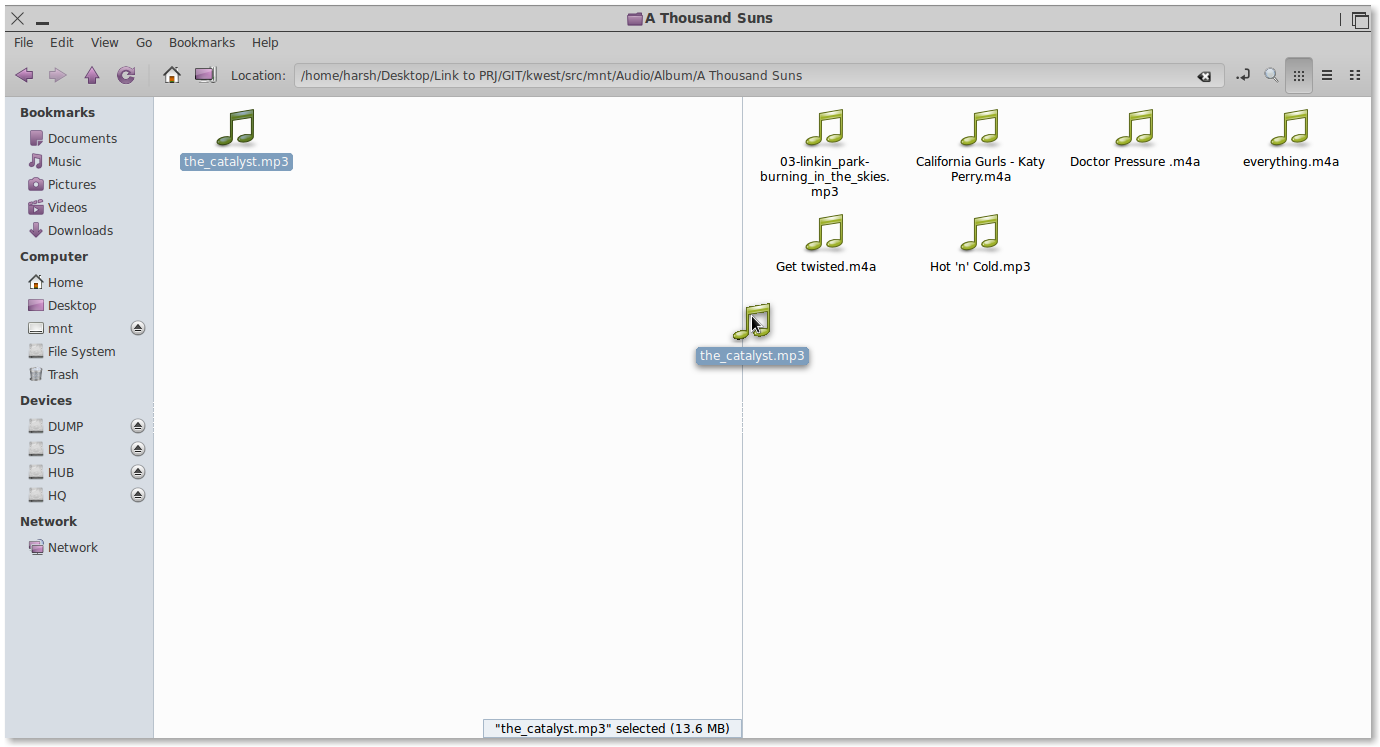
\includegraphics[width=0.8\linewidth]{./opimg/copyfile.png}}
%\includegraphics[width=0.8\textwidth]{image.png}
\caption{Copying files to/from/within KWEST}
\label{fig:dfd0}
\end{figure}
%5. Delete
\item \textbf{Delete files:}
Deleting a file causes that file to be untagged from the current tag. When all instances of a file have been untagged, i.e. a file is no longer tagged under any tag, it is removed from the database.
\end{itemize}

\subsection{Permissions:}
File/Folder permissions allow the user to control who has access to their data and how much they can interact with it. KWEST uses the underlying system permissions to provide security from unauthorised access. Users can use the $chmod$ and $chown$ to manage these permissions. KWEST works perfectly with these commands to provide proper security and restrictions for the users files.

\subsection{Browsing:} 
The user can browse a KWEST file system with any tools, software which work on traditional file systems. All popular terminals, browsers, file managers work `\textit{as is}' with KWEST. 


\section{Suggestions:}
KWEST helps the user with organisation by providing suggestions for tagging files. These suggestions are provided as files prefixed with the word - ``\textit{SUGGESTED}''. The user may make use of that suggestion by tagging that file in the current tag. \newline
e.g. in tag \textit{Zodiac}, there are 3 suggestions: \textit{ARIES, GEMINI, CANCER} each shown as a file with \textit{SUGGESTED} prefixed in their names. To make use of the suggestion on \textit{ARIES}, the user tags the file \textit{ARIES} under the tag \textit{Zodiac}. The file is now seen in the tag without the suggested prefix. The other suggestions are still present and may be used further or deleted.
\begin{figure}[htb]
\centering
\setlength\fboxsep{0pt}
\setlength\fboxrule{0.5pt}
\fbox{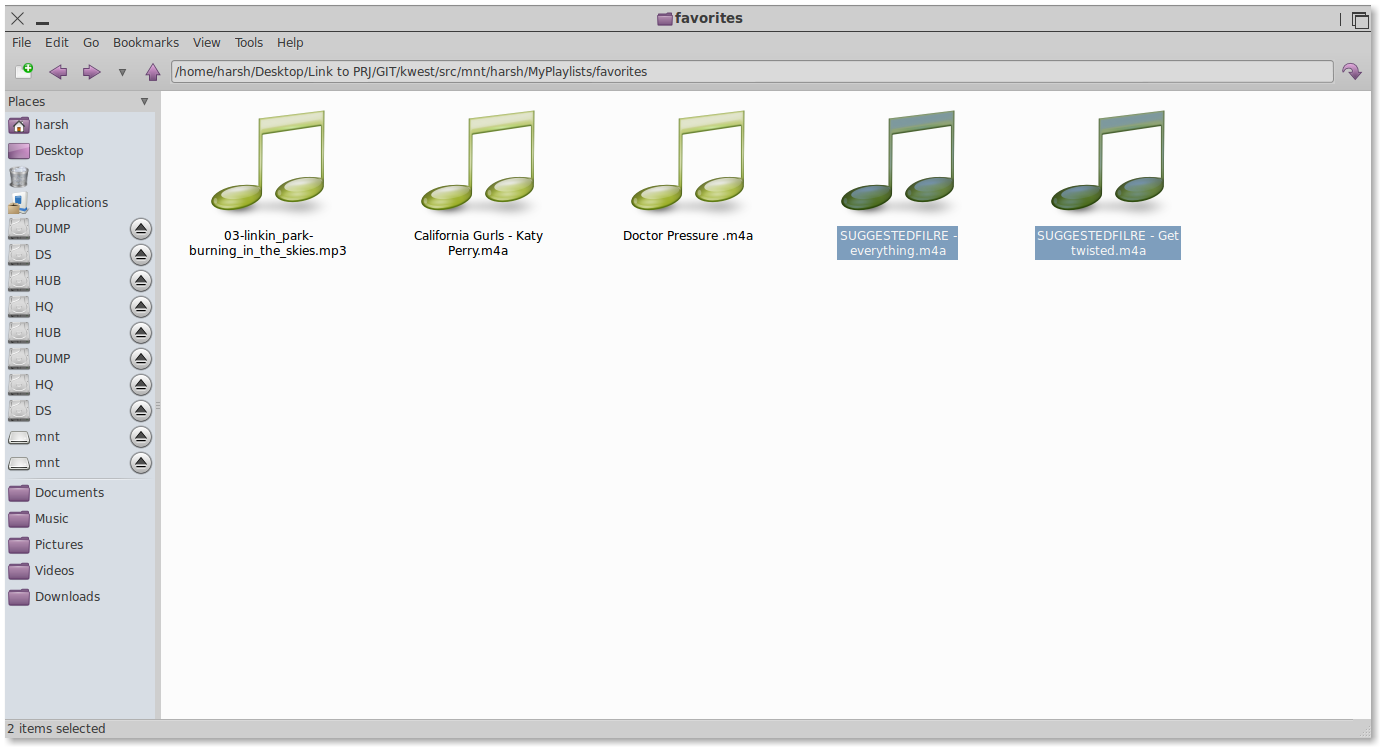
\includegraphics[width=0.8\linewidth]{./opimg/suggestions.png}}
%\includegraphics[width=0.8\textwidth]{image.png}
\caption{KWEST offering suggestions for tag favorites}
\label{fig:dfd0}
\end{figure}

\subsection*{Forming suggestions:}
Each time the file system is mounted, the system tries to generate new suggestions. These suggestions are stored in the database and are displayed when the user browses relevant tags. The suggestions are formed on the basis of the \textit{Apriori} algorithm by approximating which files are commonly tagged. If the user forms new tags and/or tags some files, the suggestions based on these changes will happen only on the next mount of the file system.

\section{F.A.Q.}
\begin{enumerate} 
\item \emph{The project won't compile. I followed the steps correctly, but there are some errors while building...} \newline
Make sure you have all the dependencies installed and they are up-to-date with the requirments. Sometimes, a system error may interfere in the installation, you may want to restart and try again. The installation does not require administrative privelages, however, you must be able to execute the make file for the installation.
\item \emph{It gives some error regarding missing kw libraries. Where do I get them?} \newline
This is due to the libraries being incorrectly linked. You can retype the \textit{export} command from the installation steps.
\item \emph{The importing of files takes a long time OR is stuck on one particular file...} \newline
This may happen if that file is being kept busy by some other process. Also, for some file-types such as long videos, the extraction of metadata takes some time. You may wait for some time for the program to complete its operation or abort and restart the proess. No data is lost of corrupted by doing this.
\item \emph{I get \texttt{segmentation fault} errors and the program crashes.} \newline
This happens mostly due to file system corruption. You can try unmounting and mounting the file system again. If this still does not solve the issue, you may have to re-install or compile the program.
\item \emph{I get a \texttt{Software connection abort} error while browsing the file system.} \newline
This is mostly due to database corruption due to a file being deleted, or external interferences in the functioning of the file system. If the above said steps do not work, you may have to install it again.
\item \emph{I get a \texttt{Operation not permitted} error.} \newline
This error occurs whenever the user tries to perform some operations restricted by the KWEST file system. Such as copying from Audio to Images. The file system specifies that this operation is not permitted.
\item \emph{I get a \texttt{Transport endpoint not connected} error after mounting the file system.} \newline
This error occurs when the system cannot connect or access the mounted file system. Check whether you have correctly mounted the file system. If yes, try unmounting and mounting. If the error persists, you may have to install the program again.
\item \emph{I right-click the file system and select unmount, but it gives a system error.} \newline
Since this is a virtual file system created with FUSE, you can only unmount it using the \texttt{fusermount -u} command. See Unmounting section for more info on this.

\end{enumerate}